\section{FrameNet: Surface Parameterization from Texture}
\label{sec:framenet}
\subsection{Approach}
In this section, we develop our approach for learning local \cframe{} from RGB images. First, we discuss the ground truth labeling of \cframe{} from 2D images in section~\ref{sec:framenet-prepare-data}. Then, we discuss the concept of projected tangent principal directions in section~\ref{sec:framenet-project}. Finally in section~\ref{sec:framenet-network}, we propose several energy terms that encourage the neural network to predict consistent local \cframe{} assisted by the projected tangent principal directions. Since we focus on the behavior of the local \cframe{} rather than the neural network architecture, we can adopt any neural network that predicts per-pixel features (see experiments in Sec. \ref{sec:framenet-evaluation} and \ref{sec:framenet-applications}).

\subsubsection{Local \ccff{} Generation}
\label{sec:framenet-prepare-data}
To label the \cframe, we need a dataset with 3D meshes aligned with RGB images to compute frames from geometry and render them to images as ground truth. We choose ScanNet~\cite{dai2017scannet} for our experiments.

\begin{figure}
    \centering
    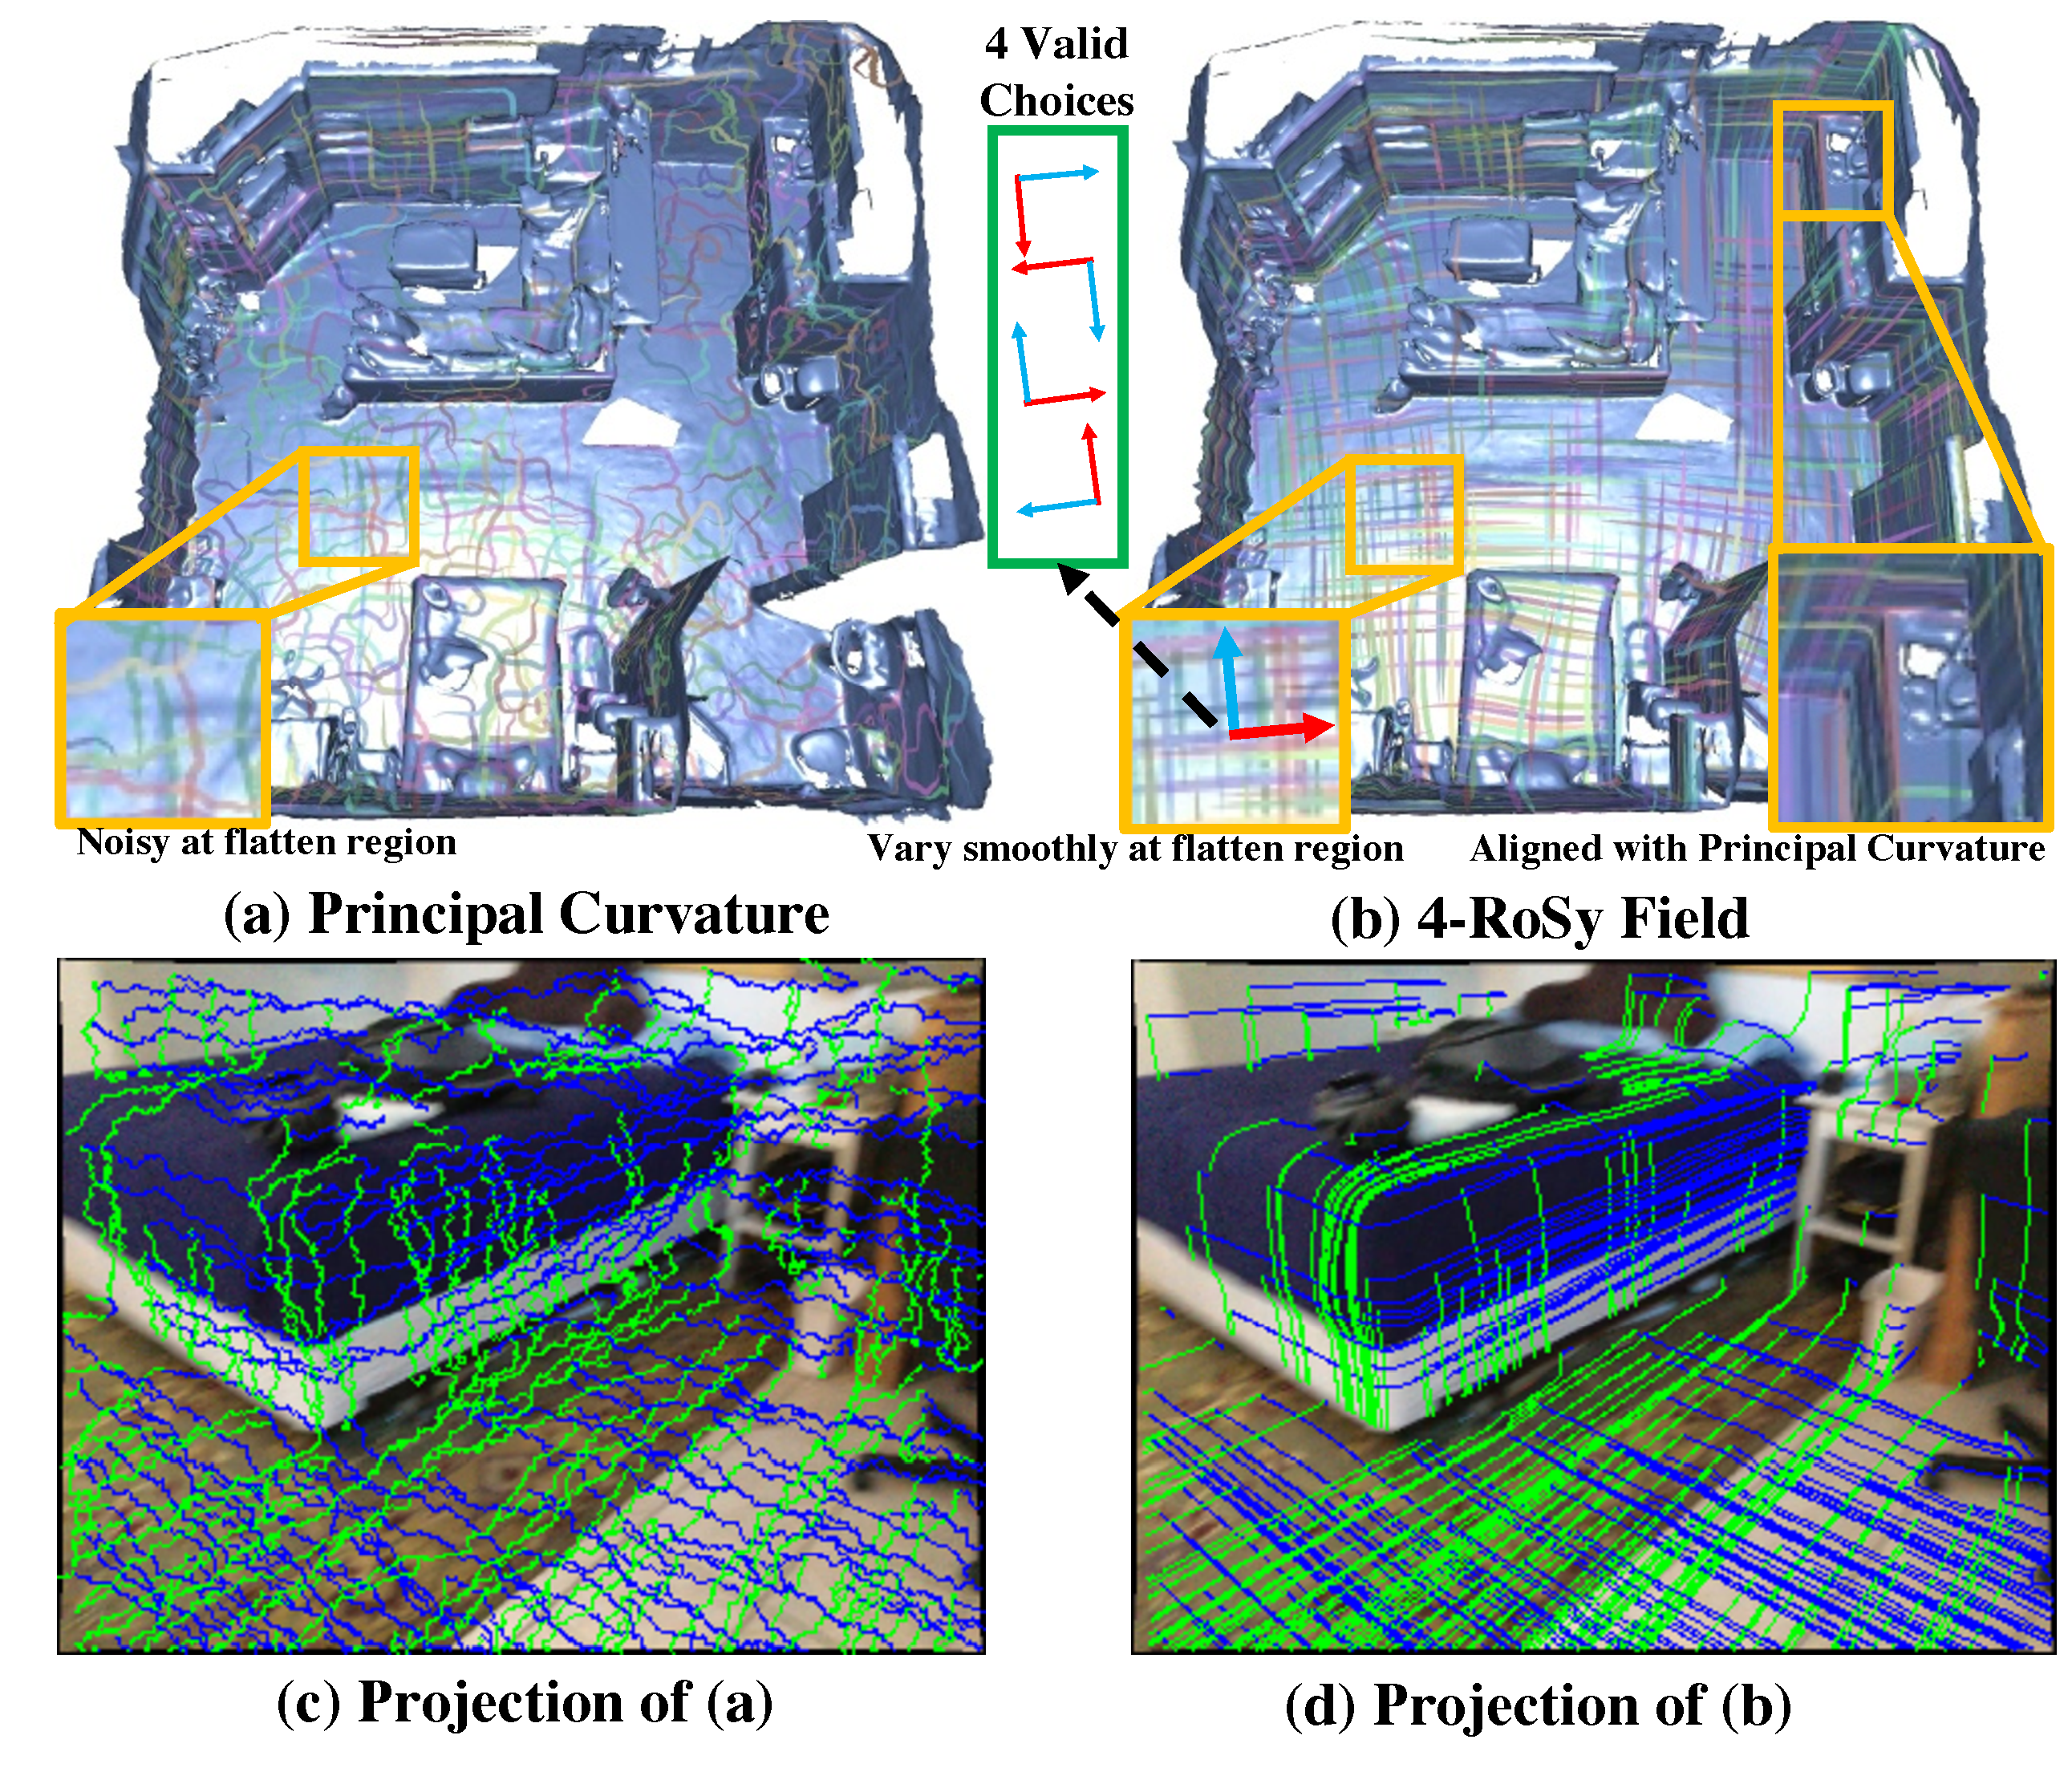
\includegraphics[width=0.8\linewidth,height=0.584\linewidth]{FrameNet/graph/4rosy.pdf}
    \vspace{-0.20in}
    \caption{(a) computes the direction field from estimated principal curvatures. Noise exists in both the geometry and the projections in images, as shown in (c). (b) computes the 4-RoSy field using QuadriFlow~\cite{huang2018quadriflow} and produces robust tangent principal directions, as shown in (d) as the projection in the image plane.}
    \label{fig:framenet-vis-geometry}
\vspace{-0.1in}
\end{figure}

We compute \cframe{} as surface normals and tangent principal directions with the scene geometry. It is straightforward to compute surface normals, but tangent principal directions at flat regions are hard to compute especially in the presence of noise. As visualized in figure~\ref{fig:framenet-vis-geometry}(a,c), the tangent principal directions can be pretty noisy. To solve this problem, we adopt the 4-RoSy field using QuadriFlow~\cite{huang2018quadriflow} as proposed by TextureNet~\cite{huang2018texturenet}, as shown in figure~\ref{fig:framenet-vis-geometry}(b,d): This field generates consistent directions which vary smoothly at flatter regions and are aligned with the principal curvatures at curved surfaces. The cross-field is 4-RoSy since there are four valid choices for the tangent principal directions at each vertex. Considering this, we pick any pair of orthogonal tangent vectors in the cross field to represent the principal directions, but we also view the other three alternatives as valid ground truth.

\begin{figure}
    \centering
     \begin{minipage}{0.19\linewidth}
     \centering
     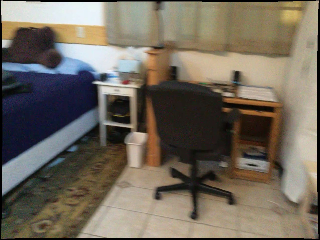
\includegraphics[width=\linewidth]{FrameNet/Dataset/pred-000001-color.png}\\
     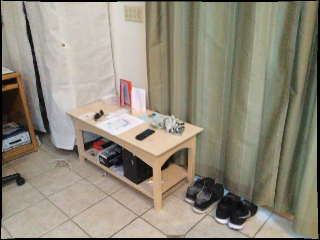
\includegraphics[width=\linewidth]{FrameNet/Dataset/pred-000003-color.png}\\
     %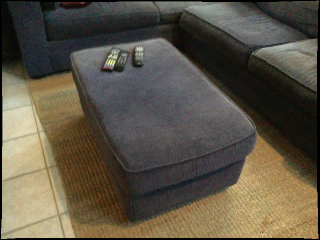
\includegraphics[width=\linewidth]{Dataset/pred-000005-color.png}\\
     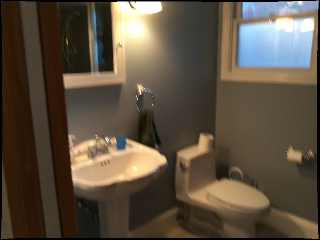
\includegraphics[width=\linewidth]{FrameNet/Dataset/pred-000021-color.png}\\
     \vspace{-0.05in}
     RGB
    \end{minipage}
     \begin{minipage}{0.19\linewidth}
     \centering
     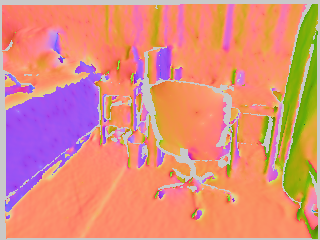
\includegraphics[width=\linewidth]{FrameNet/Dataset/pred-000001-X.png}\\
     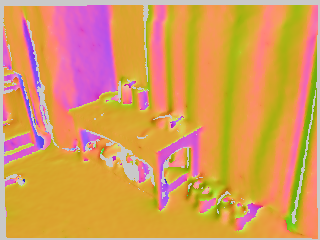
\includegraphics[width=\linewidth]{FrameNet/Dataset/pred-000003-X.png}\\
     %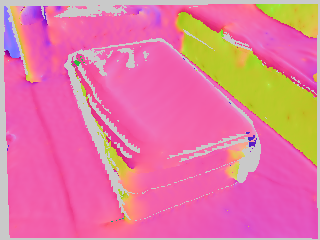
\includegraphics[width=\linewidth]{Dataset/pred-000005-X.png}\\
     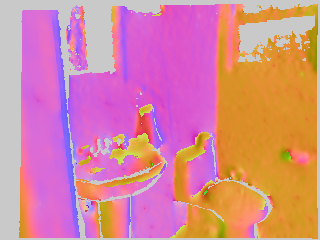
\includegraphics[width=\linewidth]{FrameNet/Dataset/pred-000021-X.png}\\
     \vspace{-0.05in}
     X
    \end{minipage}
     \begin{minipage}{0.19\linewidth}
     \centering
     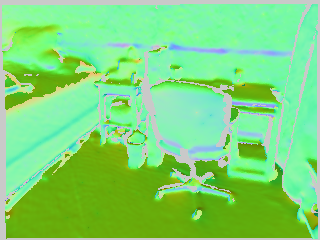
\includegraphics[width=\linewidth]{FrameNet/Dataset/pred-000001-Y.png}\\
     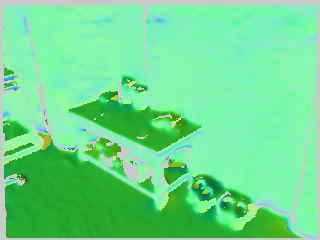
\includegraphics[width=\linewidth]{FrameNet/Dataset/pred-000003-Y.png}\\
     %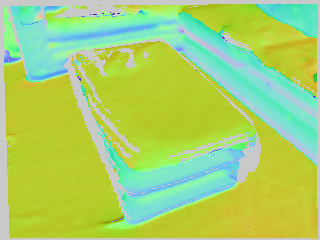
\includegraphics[width=\linewidth]{Dataset/pred-000005-Y.png}\\
     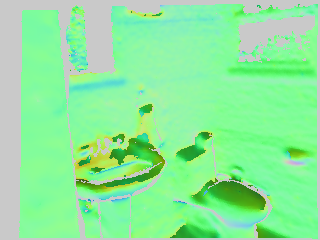
\includegraphics[width=\linewidth]{FrameNet/Dataset/pred-000021-Y.png}\\
     \vspace{-0.05in}
     Y
    \end{minipage}
     \begin{minipage}{0.19\linewidth}
     \centering
     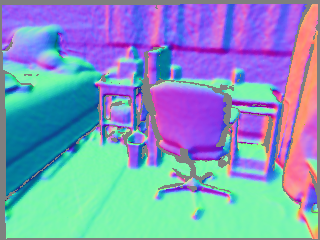
\includegraphics[width=\linewidth]{FrameNet/Dataset/pred-000001-normal.png}\\
     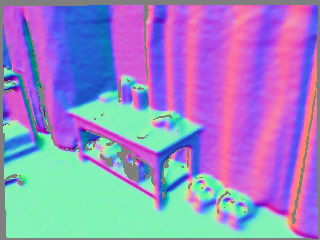
\includegraphics[width=\linewidth]{FrameNet/Dataset/pred-000003-normal.png}\\
     %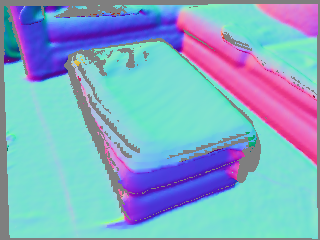
\includegraphics[width=\linewidth]{Dataset/pred-000005-normal.png}\\
     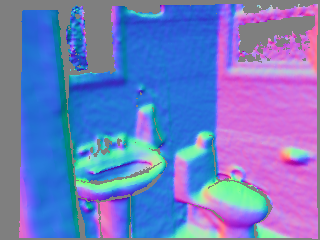
\includegraphics[width=\linewidth]{FrameNet/Dataset/pred-000021-normal.png}\\
     \vspace{-0.05in}
     Normal
    \end{minipage}
     \begin{minipage}{0.19\linewidth}
     \centering
     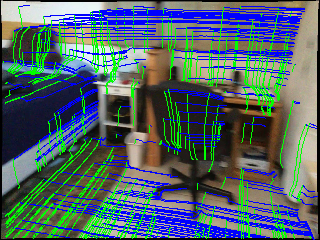
\includegraphics[width=\linewidth]{FrameNet/Dataset/pred-000001-vis-gt.png}\\
     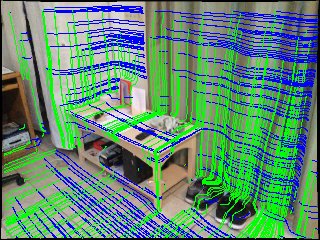
\includegraphics[width=\linewidth]{FrameNet/Dataset/pred-000003-vis-gt.png}\\
     %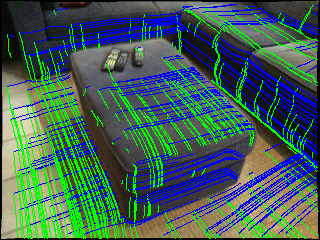
\includegraphics[width=\linewidth]{Dataset/pred-000005-vis-gt.png}\\
     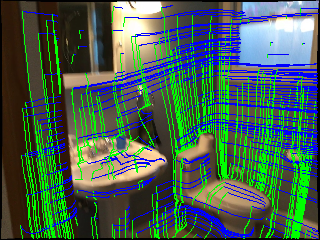
\includegraphics[width=\linewidth]{FrameNet/Dataset/pred-000021-vis-gt.png}\\
     \vspace{-0.05in}
     Projection
    \end{minipage}
    \caption{Local \ccff{} Dataset. For each RGB frame, we render the corresponding tangent principal directions (X and Y) for each pixel. The surface normal can be computed as the cross product of the principal directions.}
    \label{fig:framenet-dataset}
\vspace{-0.1in}
\end{figure}

We store the computed local \cframe{} on top of mesh vertices and render them to images after transforming them to the camera space. For each triangle to be rendered, we enumerate the $90^{\circ}N (N\in \mathbb{Z})$ degree rotations to the tangent principal directions of the last two vertices, so as to align them with the first vertex before the standard rasterization stage. This is to deal with the 4-way rotational ambiguities in the cross field. For each RGB image, we render and save the tangent principal directions as two images, as shown in figure~\ref{fig:framenet-dataset} as X and Y. The ground truth normal can be directly computed as the cross product of them.

\subsubsection{Projected Principal Directions}
\label{sec:framenet-project}
Since we aim to predict 3D principal tangent directions from their appearances into RGB images, we first derive the projective geometry that relates them.

%We observe that the projected tangent principal directions are mostly consistent with the object boundaries or image gradients as shown in figure~\ref{fig:framenet-vis-geometry}(d). Therefore, we want to study the relationship between the tangent principal directions and their projections in the image.

 For a pixel $\mb{p}=(p_x,p_y)$ in the canonical camera coordinate system, its 3D position of the pixel can be represented as $\mb{P}=(p_xd, p_yd, d)$ where $d$ is the depth value. Suppose the pixel has two tangent principal directions $\mb{i}$ and $\mb{j}$, and we want to analyze their projections. For $\mb{i}=(i_x,i_y,i_z)$, we can project a line segment $l(\mb{P},\delta,\mb{i})$ that connects endpoints $\mb{P}$ and $\mb{P}+\delta \cdot \mb{i}$ into the image as $l_p(\textbf{P},\delta,\mb{i})$, which is the offset from $\mb{p}$ to the projection of $\mb{P}+\delta \mb{i}$:
\begin{equation}
    l_p(\textbf{P},\delta,\textbf{i}) = \frac{\textbf{P}+\delta \textbf{i}}{(\textbf{P}+\delta \textbf{i})_z}-\mb{p}=(i_x - p_x i_z, i_y - p_y i_z)\frac{\delta}{d+\delta i_z}\,.
\end{equation}

We find several ways to translate the projected line segment as a property of the pixel, as shown in equation~\ref{eq:framenet-def1},\ref{eq:framenet-def2},\ref{eq:framenet-def3}. The most straightforward idea is to define the property as the projection of the unit 3D line segment from the pixel through the principal directions, represented as 
\begin{equation}
    l^1_p(\textbf{P},\textbf{i}) := l_p(\textbf{P},1,\mb{i}).
    \label{eq:framenet-def1}
\end{equation}
This simple definition, however, requires a complex mathematical form including the depth value as a hidden information. Thus it could be hard to learn. Another property is the normalized projected principal direction, or
\begin{equation}
    l^u_p(\textbf{P},\textbf{i}) := \frac{l_p(\textbf{P},\delta,\mb{i})}{||l_p(\textbf{P},\delta,\mb{i})||_2} = \frac{(i_x - p_x i_z, i_y - p_y i_z)}{||(i_x - p_x i_z, i_y - p_y i_z)||_2}.
    \label{eq:framenet-def2}
\end{equation}
This representation removes the influence of depth as the challenging hidden property. Since the projection usually aligns with the image gradients, it can be as easy as the task of predicting the normalized gradient for the neural network. However, though this is an easy task, the unit projected direction cannot determine the original 3D direction. As shown in figure~\ref{fig:framenet-dir-constraint}(a), a 2D direction in an image is corresponding to a plane in the 3D world, in which any 3D direction could be a valid solution. Fortunately, we can simplify the definition as
\begin{equation}
    l_p^*(\textbf{P},\textbf{i}) := (i_x - p_xi_z, i_y-p_yi_z).
    \label{eq:framenet-def3}
\end{equation}
This excludes the influence of the depth and gives enough supervision to the directions in 3D space. Mathematically, given the prediction of $\mb{l}_p^*(\mb{P},\mb{i})=(l^\mb{i}_x,l^\mb{i}_y)$, we can compute direction $\mb{i}=(i_x,i_y,i_z)$ by solving the system~\ref{eq:framenet-solve}:
\begin{equation}
\begin{cases}
  i_x - p_x i_z = l^\mb{i}_x\\
  i_y - p_y i_z = l^\mb{i}_y\\
  i_x^2 +i_y^2 + i_z^2 = 1\,.
\end{cases}
\label{eq:framenet-solve}
\end{equation}
\begin{figure}
    \centering
     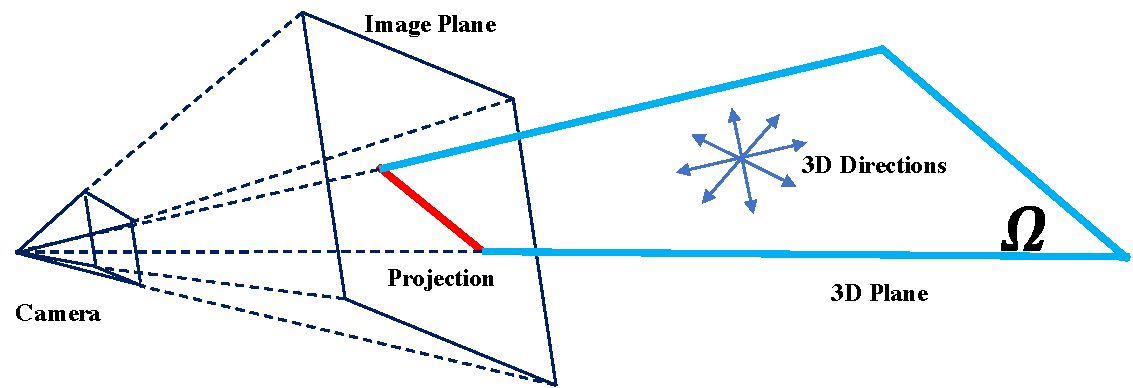
\includegraphics[width=0.8\linewidth]{FrameNet/graph/projection.pdf}
     \caption{Each projected direction in the image plane (shown in red) corresponds to a 3D plane $\Omega$ in the scene. Any 3D direction inside the plane is a valid candidate for this direction.}
    \label{fig:framenet-dir-constraint}
\vspace{-0.2in}
\end{figure}
    \vspace{-0.1in}
\subsubsection{Joint Estimation}
\label{sec:framenet-network}
We could train a network to estimate the projected principal directions $\mb{i}_p=l_p^*(\textbf{P},\textbf{i})$ and $\mb{j}_p=l_p^*(\textbf{P},\textbf{j})$, and directly infer $\mb{i}$ and $\mb{j}$ according to equation~\ref{eq:framenet-solve} for \cframe{} estimation. However, we find that this approach does not lead to a robust \cframe{}. Therefore, we propose to jointly estimate the \cframe{} as well as the projected tangent principal directions, and enforce their orthogonality and projection consistency with additional soft energy constraints.  We expect that the extra constraints will provide a regularization that can help the network learn.

\begin{figure}
    \centering
    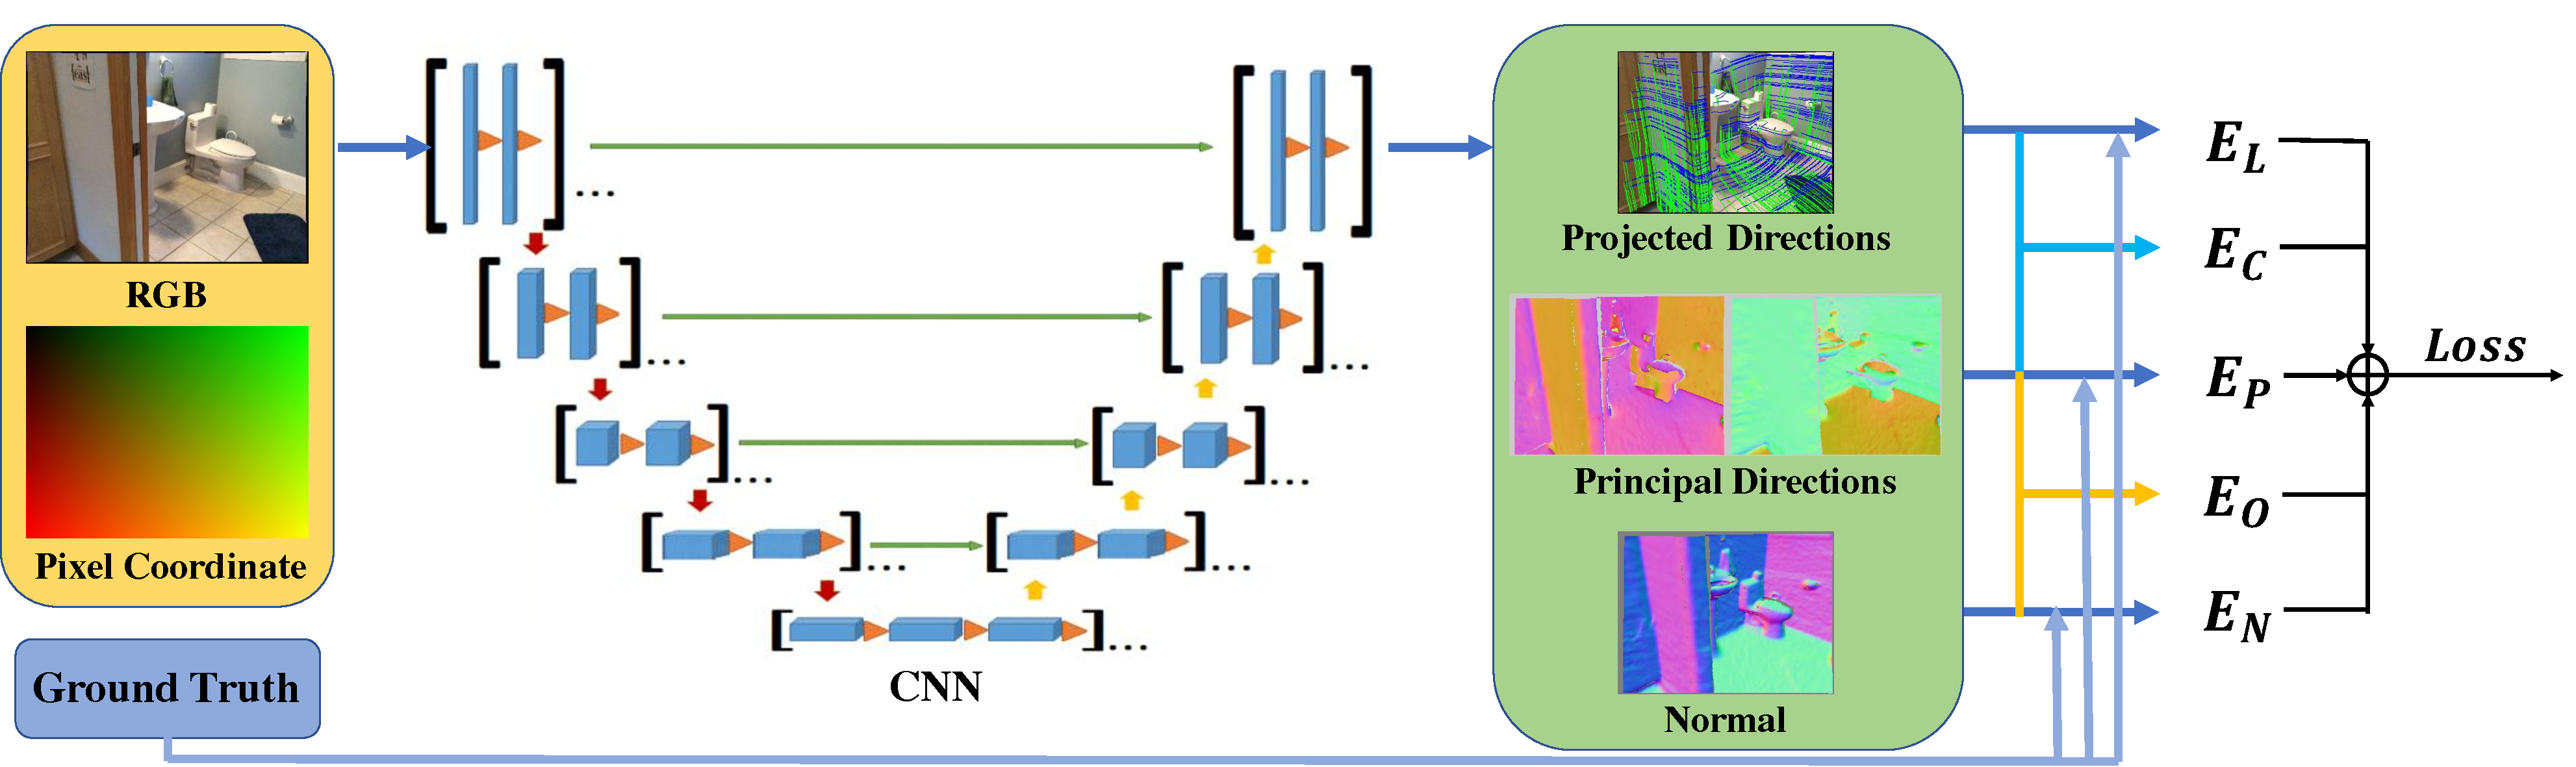
\includegraphics[width=\linewidth]{FrameNet/graph/architecture.pdf}
    \caption{To estimate the local \cframe{}, we feed the RGB image and the canonical pixel coordinate map to the network. The output is a 13-dimensional vector for each pixel including two projected tangent principal directions, two 3D tangent principal directions, and one normal vector. We propose a new loss that utilizes the projected directions to improve the estimation of the \cframe{}.}
    \label{fig:framenet-architecture}
\end{figure}
Our proposed solution is illustrated in figure~\ref{fig:framenet-architecture}. The neural network can be viewed as a black box function that predicts per-pixel features for the RGB image. Since the projected tangent principal directions relate to the pixel coordinate in the canonical camera, we feed the canonical pixel coordinate together with its RGB values into the network as the input. The network outputs a 13-dimensional vector includes two tangent principal directions $\mb{i}$ and $\mb{j}$, their 2D projections $\mb{i}_p$ and $\mb{j}_p$, and the surface normal $\mb{n}$.

We propose a set of energies so that projected tangent principal directions can assist the local principal axes estimation. The loss energy $E$ is a linear combination of five energy terms as shown in equation~\ref{eq:framenet-loss},
\begin{align}
\begin{split}
  E = \lambda_L &E_L + \lambda_P E_P + \lambda_N E_N + \lambda_C E_C + \lambda_O E_O\\
  E_L &= \min_{0\leq k \le 4} ||[\mb{i}_p,\mb{j}_p] - R_k([\mb{i}_p^{gt},\mb{j}_p^{gt}])||_2^2\\
  E_P &= \min_{0\leq k \le 4} ||[\mb{i},\mb{j}] - R_k([\mb{i}^{gt},\mb{j}^{gt}])||_2^2\\
  E_N &= ||N - N^{gt}||_2^2\\
  E_C &= ||l^*_p(\mb{i}) - \mb{i}_p||_2^2+||l^*_p(\mb{j}) - \mb{j}_p||_2^2\\
  E_O &= ||N - \mb{i}\times\mb{j}||_2^2\,, \\
\end{split}
\label{eq:framenet-loss}
\end{align}
where $R_1([\mb{a},\mb{b}])=[-\mb{b},\mb{a}]$ and $R_k = R_1\circ R_{k-1} (k>1)$.

Specifically, $E_L$ measures the distance between the predicted tangent principal directions and the ground truth in the 2D projected space. $R_k$ represents the $90^{\circ}k$ degree rotation around the normal axis. $E_L$ removes the rotational ambiguity by enumerating the possible $90^{\circ}k$ rotations and measure the minimum L2 loss among them. Similarly, $E_P$ measures the minimum L2 loss of tangent principal directions in the 3D space, and $E_N$ measures the L2 loss of the surface normal estimation. In order to connect the tangent principal directions to their projections, we design $E_C$ to measure the consistency between the projected predicted directions ($l^*_p(\mb{i})$,$l^*_p(\mb{j})$) and the predicted one ($\mb{i}_p$,$\mb{j}_p$) by the network. Finally, we also hope the influence can be propagated to the surface normal, so we add an orthogonality constraint $E_O$ to enforce that the surface normal is orthogonal to the tangent principal directions.

Since all the distances are roughly on the same scale, we set $\lambda_L=\lambda_P=\lambda_N=1$ to balance the penalty for errors for different vectors. To enforce the system to predict orthogonal \cframe{} with consistent 2D projection, we set $\lambda_C=\lambda_O=5$ in our experiments to provide slightly stronger constraints between network predictions.

\subsection{Evaluation}
\label{sec:framenet-evaluation}
In this section, we describe a series of experiments to evaluate our method for local \cframe{} estimation and do ablation studies using the ScanNet dataset~\cite{dai2017scannet}. 
Unless otherwise specified, we used the DORN architecture~\cite{fu2018deep} as the backbone for the architecture in fig. \ref{fig:framenet-architecture}, and we used equation~\ref{eq:framenet-def3} for the projected tangent principal directions, since they gave the best results (see below).
The main conclusion of these tests is that jointly predicting the projected tangent directions and enforcing the consistency loss are major contributors to the success of local principal axes and surface normal estimation.

%We did experiments to understand the network's ability to learn different proposals of our projected tangent principal directions. We are also interested in studying the behavior of the predicted terms and losses. 
%Our experiments show that the proposed formulations in equation~\ref{eq:framenet-def2} and \ref{eq:framenet-def3} achieve similar errors and significantly outperform equation~\ref{eq:framenet-def1}. We also find that projected tangent directions and the consistency loss are major contributors to the success of local principal axes estimation.

\vspace{-0.1in}
\paragraph{How well can canonical frames be estimated from RGB?}  Our first experiment simply investigates how well our algorithm can predict the \cframe{}.   Since this is a new task, there is no suitable comparison to prior work.   However, we can still gain insight into the problem by comparing errors in predicted normals, principal tangent principal directions, and projected tangent principal directions.   The results in table~\ref{tab:framenet-3dframe} show that prediction of projected tangent principal directions have least error, surface normals have most error, and tangent principal directions are in the middle.   This suggests that predicting tangent directions is less error prone than normals, which should be expected since they largely align with textures and gradients in the input image (figure~\ref{fig:framenet-project}). 

\begin{table}[t]
    \centering
    \small
    \tabcolsep=0.12cm
    \begin{tabular}{|c|c|c|c||c|c|c|}
        \hline
         \textbf{3D Frame} & mean & median & rmse & $11.25^\circ$ & $22.5^\circ$ & $30^\circ$\\
         \hline
         Normal & 15.28 & 8.14 & 23.36 & 60.6 & 78.6 & 84.7\\
         \hline
         Principal & 12.26 & 7.88 & 16.85 & 63.7 & 84.3 & 90.8\\
         \hline
         Projection & 7.55 & 4.46 & 11.36 & 79.8 & 93.0 & 96.3\\
         \hline
    \end{tabular}
    \caption{Testing mean average error of local principal axes estimation on ScanNet~\cite{dai2017scannet}. We evaluate surface normals, tangent principal directions their projections predicted by our network.}
    \label{tab:framenet-3dframe}
    %\vspace{-0.1in}
\end{table}

\begin{figure}[t]
    \centering
    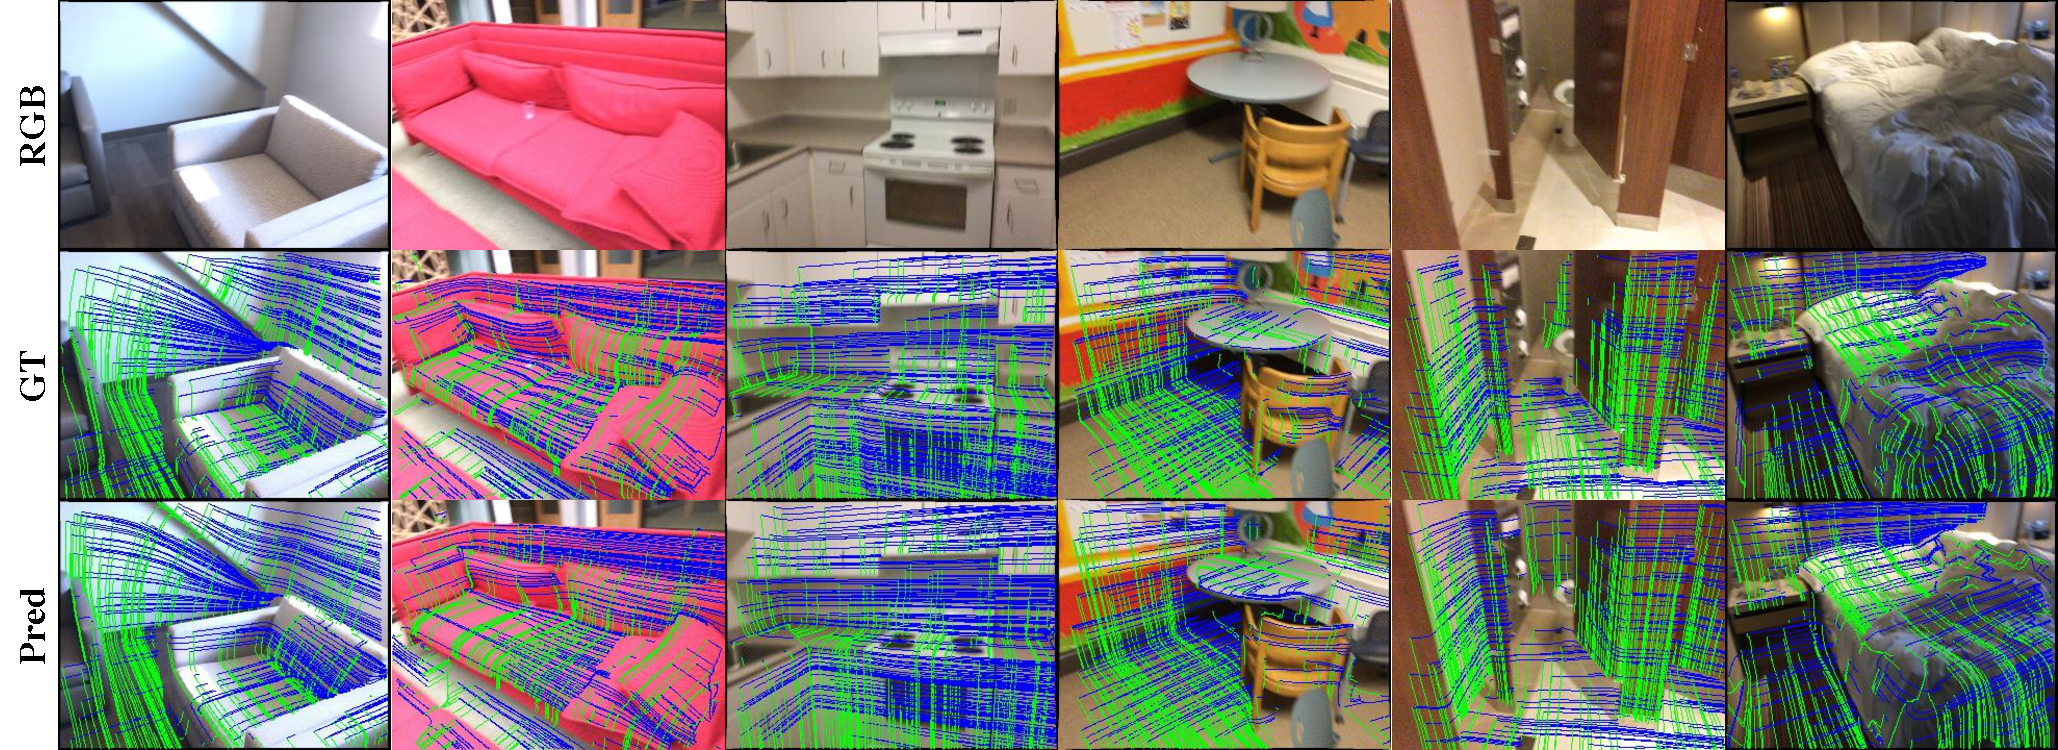
\includegraphics[width=\linewidth]{FrameNet/graph/result-ours.pdf}
    \caption{Visualization of the projected principal directions. Our estimation is similar to the ground truth at curved surfaces or texture smooth regions. The predicted directions align with textures and gradients in the input image.}
    \label{fig:framenet-project}
    %\vspace{-0.1in}
\end{figure}

\begin{table}
    \centering
    \small
    \begin{tabular}{|c|c|c|c|c|c|}
        \hline
         Method & UNet & SkipNet & GeoNet & DORN\\
         \hline
         Normal & 21.08 & 20.84 & 20.37 & 16.42\\
         \hline
         Normal-YZ & 17.49 & 17.17 & 16.71 & 12.51\\
         \hline
         Normal-XZ & 18.05 & 17.16 & 17.68 & 13.00\\
         \hline
         Normal-XY & 29.05 & 29.71 & 29.08 & 22.57\\
         \hline
         Principal & 17.55 & 15.78 & 15.41 & 12.53\\
         \hline
         Principal-YZ & 21.15 & 21.96 & 20.61 & 16.19\\
         \hline
         Principal-XZ & 22.67 & 21.87 & 21.57 & 16.65\\
         \hline
         Principal-XY & 11.47 & 9.96 & 9.53 & 7.55\\
         \hline
    \end{tabular}
    \caption{Mean angle errors of normals and tangent principal directions and their projections to three orthogonal planes on ScanNet.}
    \label{tab:framenet-error}
    %\vspace{-0.05in}
\end{table}
\label{sec:framenet-ablate}

%\vspace{-0.1in}
\paragraph{Which frame directions are easiest to predict?}  To further investigate the relative challenge of predicting different components of the local \cframe{}, we perform experiments in which we separately train normals and tangent principal directions in 3D space with L2 losses and evaluate them with mean angle errors of their projections to three planes in camera space, as illustrated in figure~\ref{fig:framenet-err-proj}.  The prediction errors and their projected components, listed in table~\ref{tab:framenet-error}, suggest
that the errors of the tangent principal directions are less than those of normals, and the projected errors on the image plane are smaller than those on the other two planes for tangent principal directions.  This again suggests that the network can predict tangent principal directions better than surface normals, especially for the components projected into the image plane.  Interestingly, the projected errors for the normal in the image plane is the largest, which might be because the network learns tangent principal directions in the latent space and propagates the errors from XZ and YZ planes to the image plane by the cross product.
\begin{figure}
    \centering
    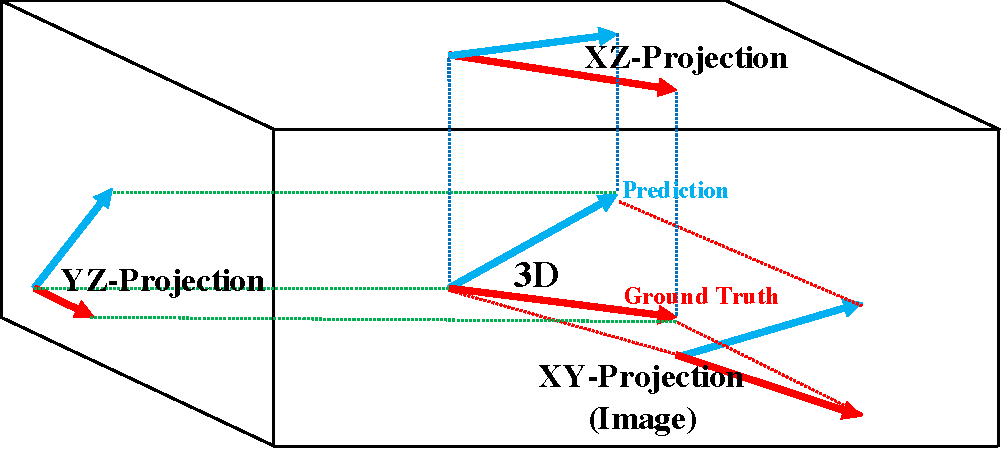
\includegraphics[width=0.6\linewidth]{FrameNet/graph/angleproj.pdf}
    \caption{By projecting the directions into XY, YZ, XZ planes in the camera space, we can measure the projected angle error.}
    \label{fig:framenet-err-proj}
%\vspace{-0.1in}
\end{figure}


%\vspace{-0.1in}
\paragraph{How does each loss contributes to the estimation?}
We next study how our proposed consistency losses influence the learning process. In table~\ref{tab:framenet-consistency}, we present the testing mean average angle for surface normals w/o. certain parts of losses during training on ScanNet. We note that by directly predicting all $E_N$ and $E_P$ together, there is already an improvement. The reason could be that the correlation between predicted principal directions and the 3D frames are automatically learned from the data distribution. However, the improvement is minor without predicting the projected principal directions with $E_L$. With orthogonal or consistency constraints, the performance can be further improved and achieve maximum with both.
\begin{table}
    \centering
    \tabcolsep=0.20cm
    \small
    \begin{tabular}{|c|c|c|c|c|c|}
        \hline
         Method & UNet & SkipNet & GeoNet & DORN\\
         \hline
         $E_N$ & 21.08 & 20.36 & 19.77 & 16.42\\
         \hline
         $E_N$,$E_P$ & 21.04 & 20.45 & 19.64 & 16.29\\
         \hline
         $E_N$,$E_P$,$E_L$ & 20.62 & 19.47 & 19.26 & 15.45\\
         \hline
         $E_N$,$E_P$,$E_L$,$E_O$ & 20.58 & 19.43 & 19.18 & 15.41\\
         \hline
         $E_N$,$E_P$,$E_L$,$E_C$ & 19.79 & 19.44 & 19.02 & 15.31\\
         \hline
         All Losses & \textbf{19.68} & \textbf{19.39} & \textbf{18.96} & \textbf{15.28}\\
         \hline
    \end{tabular}
    \caption{We test mean average angle errors for surface normal predictions with different combination of loss terms on ScanNet. $E_L$ and $E_C$ has major contributions to the improvement, suggesting the importance of the projected principal directions.}
    \label{tab:framenet-consistency}
    %\vspace{-0.1in}
\end{table}

\vspace{-0.1in}
\paragraph{Does the method generalize to different networks?}  To study the generality of our approach, we tested it with different network architectures.   Table~\ref{tab:framenet-consistency} shows that our joint losses improve performance for all the tested networks including UNet\cite{ronneberger2015u}, SkipNet\cite{bansal2016marr}, GeoNet\cite{qi2018geonet} and DORN\cite{fu2018deep}.

\vspace{-0.1in}
\paragraph{Which definition of projected directions is best?}
In equation~\ref{eq:framenet-def1}~\ref{eq:framenet-def2}~\ref{eq:framenet-def3}, we propose three choices for projected tangent principal directions. We use UNet~\cite{ronneberger2015u} to separately train and test them on ScanNet~\cite{dai2017scannet} as shown in table~\ref{tab:framenet-def}. The mean angle error for equation~\ref{eq:framenet-def1} is the highest as a complex function related to the depth. The error for equation~\ref{eq:framenet-def3} is only slightly higher than that in equation~\ref{eq:framenet-def2}, but equation~\ref{eq:framenet-def3} can explicitly guide the 3D directions with the consistency loss $E_C$. Therefore, we select equation~\ref{eq:framenet-def3} together with the canonical frames for joint estimation.

\begin{table}[t]
    \centering
    \tabcolsep=0.13cm
    \small
    \begin{tabular}{|c|c|c|c||c|c|c|}
        \hline
         \textbf{ScanNet} & mean & median & rmse & $11.25^\circ$ & $22.5^\circ$ & $30^\circ$\\
         \hline
         $l^1_p(\mb{P},\mb{i})$ & 11.13 & 7.63 & 15.00 & 65.1 & 86.2 & 92.5\\
         \hline
         $l^u_p(\mb{P},\mb{i})$ & \textbf{7.35} & \textbf{4.38} & \textbf{10.94} & \textbf{81.2} & \textbf{93.6} & \textbf{96.7}\\
         \hline
         $l^*_p(\mb{P},\mb{i})$ & 7.56 & 4.46 & 11.36 & 79.8 & 93.0 & 96.3\\
         \hline
    \end{tabular}
    \caption{Testing mean average error of different choices for projected tangent principal directions on ScanNet dataset.}
    \label{tab:framenet-def}
%\vspace{-0.15in}
\end{table}

\subsection{Applications}
\label{sec:framenet-applications}

In this section, we investigate whether the estimation of local \cframe{} is useful for applications.   We first study surface normal estimation, a direct application of our method.   In addition, we study how 3D \cframe{} can be utilized for perspective invariant feature descriptors and augmented reality.

\subsubsection{Surface Normal Estimation}
\label{sec:framenet-normal}
%\jw{We show that the joint estimation can lead to an improvement in normal estimation, although we are solving a harder task than normal estimation. The reason could be that} we force the network to understand the underlying geometry more deeply. Our network can be transferred to NYUv2 while beating the state-of-the-art.

\paragraph{Test on ScanNet}
We first compare the performance of our surface normal estimation with state-of-the-art methods on ScanNet~\cite{dai2017scannet}. 
%We pick ScanNet~\cite{dai2017scannet} and SunCG~\cite{song2015sun} as two datasets for comparison since they provided us the image-to-mesh alignment, where the ground truth local \cframe{} can be automatically computed. 
We use our approach to train four networks and evaluate them according to ground truth provided by RGBD. Table~\ref{tab:framenet-scannet-comparison} shows the results for all networks including UNet~\cite{ronneberger2015u}, SkipNet~\cite{bansal2016marr}, GeoNet~\cite{qi2018geonet} and DORN~\cite{fu2018deep}. With the assistance of the projected tangent principal directions, the normal prediction is better for all architectures.

\begin{table}
    \centering
    \tabcolsep=0.08cm
    \small
    \begin{tabular}{|c|c|c|c||c|c|c|}
        \hline
         \textbf{ScanNet} & mean & median & rmse & $11.25^\circ$ & $22.5^\circ$ & $30^\circ$\\
         \hline
         UNet & 21.08 & 14.21 & 28.55 & 40.8 & 66.9 & 76.3\\
         \hline
         UNet-Ours & 19.68 & 12.43 & 27.58 & 46.1 & 70.6 & 78.8\\
         \hline
         SkipNet & 20.36 & 13.74 & 28.63 & 45.4 & 68.2 & 77.4\\
         \hline
         SkipNet-Ours & 19.39 & 10.85 & 27.52 & 53.2 & 72.7 & 79.3\\
         \hline
         GeoNet & 19.77 & 11.34 & 28.51 & 49.7 & 70.4 & 77.7\\
         \hline
         GeoNet-Ours & 18.96 & 9.84 & 27.29 & 54.6 & 73.5 & 80.1\\
         \hline
         DORN & 16.42 & 8.64 & 24.94 & 58.7 & 76.7 & 82.9\\
         \hline
         DORN-Ours & \textbf{15.28} & \textbf{8.14} & \textbf{23.36} & \textbf{60.6} & \textbf{78.6} & \textbf{84.7}\\
         \hline         
         %\multicolumn{7}{c}{}\\
         %\hline
         %\textbf{SunCG} & mean & median & rmse & $11.25^\circ$ & $22.5^\circ$ & $30^\circ$\\
         %\hline
         %UNet & 14.88 & 6.20 & 24.94 & 64.4 & 78.6 & 83.9\\
         %\hline
         %UNet-Ours & 13.25 & 4.64 & 23.73 & 69.8 & 81.6 & 86.1\\
         %\hline
         %SkipNet & 13.38 & 3.97 & 24.54 & 70.2 & 80.3 & 85.1\\
         %\hline
         %SkipNet-Ours & 12.82 & 3.87 & 23.69 & 71.0 & 80.2 & 86.1\\
         %\hline
         %GeoNet & 13.14 & 3.56 & 23.54 & 70.6 & 80.7 & 86.0\\
         %\hline
         %GeoNet-Ours & 12.68 & 3.60 & \textbf{22.73} & 71.2 & 81.3 & \textbf{86.6}\\
         %\hline
         %DORN & 12.90 & 3.36 & 24.12 & 71.3 & 81.3 & 85.3\\
         %\hline
         %DORN-Ours & \textbf{12.38} & \textbf{3.33} & 23.34 & \textbf{72.3} & \textbf{82.3} & 86.3\\
         %\hline         
    \end{tabular}
    \caption{Evaluation on Surface Normal Predictions. We train and test our algorithm with different network architectures on the ScanNet~\cite{dai2017scannet} dataset. Assisted by our joint loss, the performances of all networks are improved.}
    \label{tab:framenet-scannet-comparison}
\end{table}

Figure~\ref{fig:framenet-vis-result} visualizes the normals predicted using DORN with and without our method. With our approach, the errors are smaller especially at object boundaries, possibly because of the additional supervision given by the projected tangent principal directions.
\begin{figure}
    \centering
    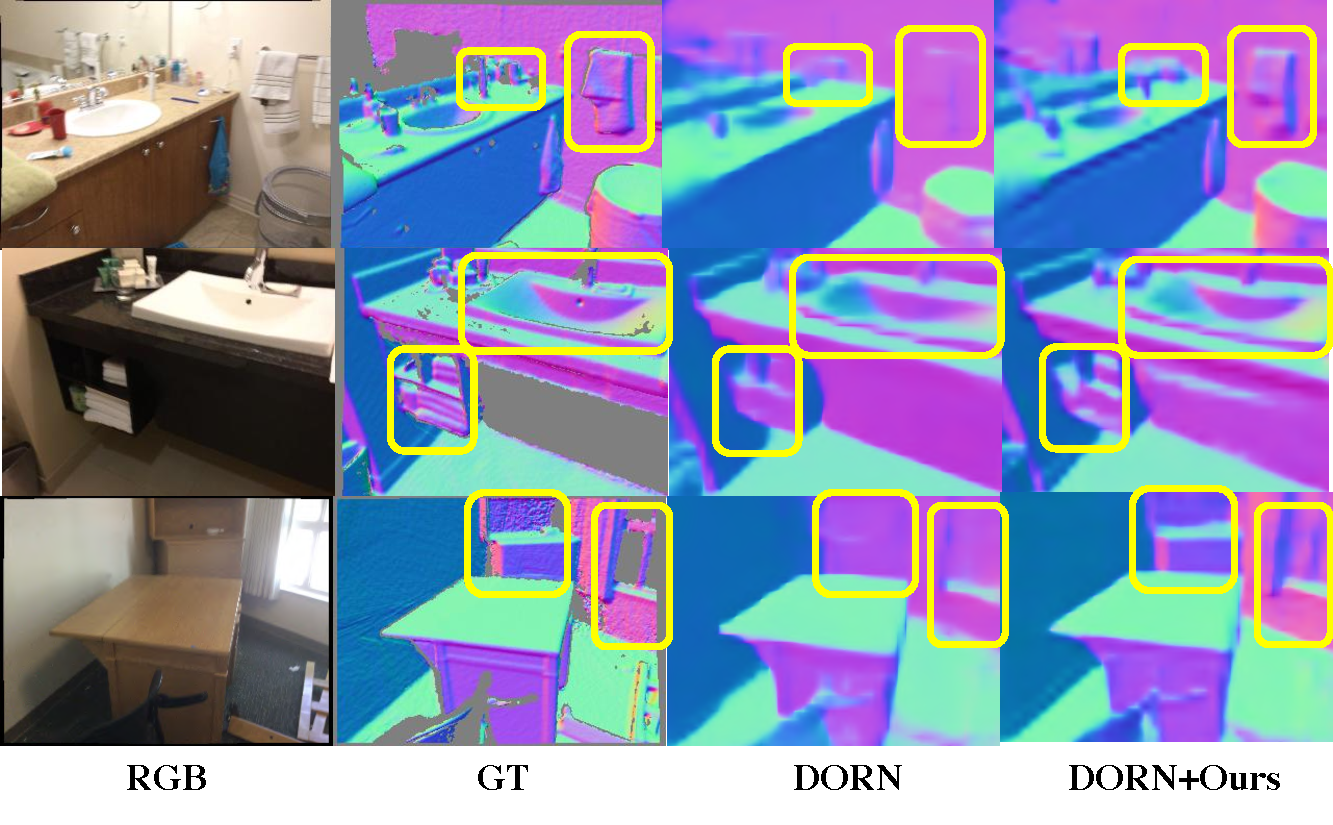
\includegraphics[width=0.8\linewidth]{FrameNet/graph/norm-compare.pdf}
    \caption{Visual comparison of the results. With our joint loss, the predicted surface normals produce less errors and more details.}
    \label{fig:framenet-vis-result}
\end{figure}

\paragraph{Test on NYUv2}
\label{sec:framenet-transfer}
We test different versions of our network on NYUv2~\cite{eigen2014depth} as a standard evaluation dataset. Since NYUv2 does not provide reconstructed 3D meshes, we cannot get ground truth 3D frames. Therefore, we train the network on ScanNet datasets and directly test on NYUv2, as shown in Table~\ref{tab:framenet-vis-nyu}. Note that GeoNet-origin~\cite{qi2018geonet} is specifically trained and tested on NYUv2 and is the current state-of-the-art method on normal estimation for that dataset. Other rows are networks trained with and without our joint losses on ScanNet and tested on NYUv2. 

\begin{table}
    \centering
    \tabcolsep=0.07cm
    \small
    \begin{tabular}{|c|c|c|c||c|c|c|}
        \hline
         \textbf{NYUv2} & mean & median & rmse & $11.25^\circ$ & $22.5^\circ$ & $30^\circ$\\
         \hline
         GeoNet-origin & 19.0 & 11.8 & 26.9 & 48.4 & 71.5 & \textbf{79.5}\\
         \hline
         \hline
         \textbf{ScanNet} & mean & median & rmse & $11.25^\circ$ & $22.5^\circ$ & $30^\circ$\\
         \hline
         UNet & 23.46 & 17.58 & 29.90 & 29.9 & 60.9 & 72.7\\
         \hline
         UNet-Ours & 22.09 & 15.45 & 29.26 & 36.9 & 64.5 & 74.9\\
         \hline
         SkipNet & 22.27 & 14.25 & 30.60 & 42.0 & 64.8 & 73.5\\
         \hline
         SkipNet-Ours & 20.68 & 13.42 & 28.33 & 46.3 & 67.4 & 76.0\\
         \hline
         GeoNet & 22.02 & 14.55 & 29.79 & 40.7 & 64.9 & 73.9\\
         \hline
         GeoNet-Ours & 20.22 & 13.23 & 28.19 & 47.9 & 68.0 & 76.4\\
         \hline
         DORN & 19.12 & 11.60 & 27.06 & 49.0 & 70.6 & 78.5\\
         \hline
         DORN-Ours & \textbf{18.63} & \textbf{11.16} & \textbf{26.61} & \textbf{50.2} & \textbf{71.6} & \textbf{79.5}\\
         \hline         
        %\hline
         %\textbf{SunCG} & mean & median & rmse & $11.25^\circ$ & $22.5^\circ$ & $30^\circ$\\
         %\hline
         %UNet & 25.21 & 18.26 & 32.82 & 32.2 & 57.7 & 68.3\\
         %\hline
         %UNet-Ours & 24.64 & 17.10 & 32.65 & 35.0 & 59.6 & 69.5\\
         %\hline
         %SkipNet & 24.75 & 17.36 & 32.45 & 33.8 & 58.1 & 69.0\\
         %\hline
         %SkipNet-Ours & 23.67 & 16.28 & 31.72 & 36.1 & 62.2 & 72.7\\
         %\hline
         %GeoNet & 22.32 & 14.97 & 30.59 & 39.8 & 64.3 & 73.4\\
         %\hline
         %GeoNet-Ours & 22.15 & 14.41 & 30.18 & 40.1 & 65.3 & 74.4\\
         %\hline
         %DORN & 22.19 & 14.46 & 30.16 & 40.3 & 65.3 & 74.1\\
         %\hline
         %DORN-Ours & 21.99 & 14.29 & 29.87 & 40.5 & 65.8 & 74.6\\
         %\hline         
    \end{tabular}
    \caption{Normal prediction on NYUv2~\cite{eigen2014depth}. GeoNet-origin trained and tested on NYUv2~\cite{qi2018geonet}.  DORN-Ours trained on ScanNet performs best among all.}
    \label{tab:framenet-vis-nyu}
\vspace{-0.1in}
\end{table}

Although GeoNet performs worse than GeoNet-origin by training only on ScanNet without fine-tuning, we still achieve better performance with the DORN~\cite{fu2018deep} architecture and our loss (DORN-Ours). Moreover, all networks show better performance with our loss, implying a robust advantage of our joint estimation. 

\subsubsection{Keypoint Matching}

Predicting local transformations is important for 
keypoint feature matching~\cite{lowe2004distinctive,bay2006surf,tola2010daisy,han2015matchnet,zagoruyko2015learning,simo2015discriminative,yi2016lift}. 
%Local feature descriptor extraction is important for keypoint matching~\cite{lowe2004distinctive,bay2006surf,tola2010daisy,han2015matchnet,zagoruyko2015learning,simo2015discriminative,yi2016lift}. 
%Recently, deep learning-based methods have been proposed~\cite{}. Among them, LIFT~\cite{yi2016lift} is currently the state-of-the-art method which offers robust feature matching.  
For example, SIFT~\cite{lowe2004distinctive} estimates scale and camera-plane rotations to provide invariance to those transformations.  Since
our network estimates a full local 3D \cframe{}, we can additionally estimate a projective warp.  
%We estimate the canonical tangent plane of the surface at each pixel and use it to warp its neighborhood before computing its descriptor, as illustrated in figure~\ref{fig:framenet-warp}.
Specifically, predicting the pairs of projected tangent principal directions (in equation~\ref{eq:framenet-def3}) for pixel $\mb{p}$ as $\mb{i}_p$ and $\mb{j}_p$ the local patch $\mathbb{P}$ is warped to $\mathbb{P}^*$ as shown in equation~\ref{eq:framenet-warp}:
\begin{equation}
    \mathbb{P}^*(\textbf{x}) = \mathbb{P}([\textbf{i}_p, \textbf{j}_p]\textbf{x})\,.
    \label{eq:framenet-warp}
\end{equation}

\begin{figure}[t]
\centering
    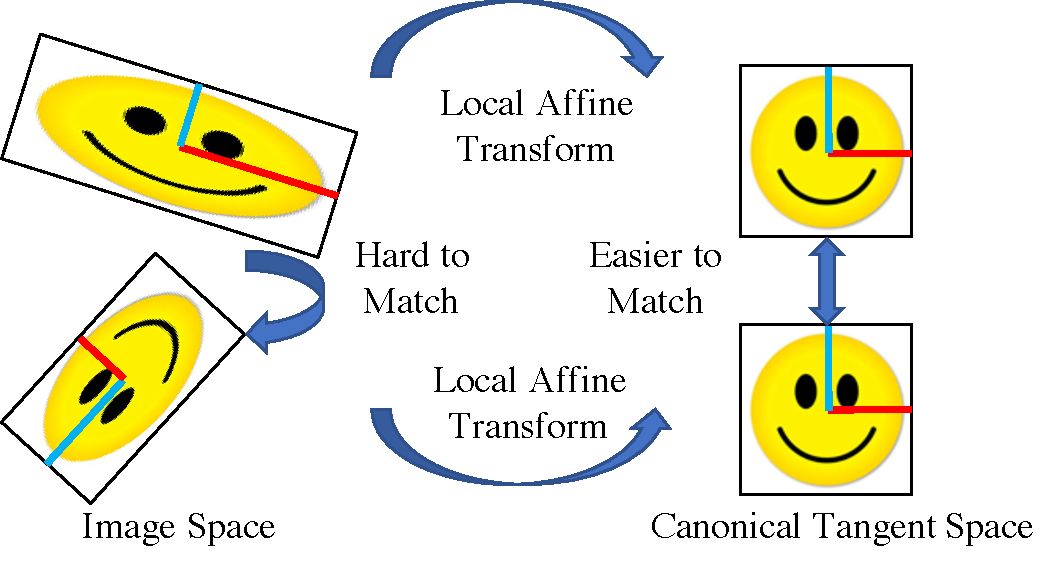
\includegraphics[width=0.7\linewidth]{FrameNet/graph/match.pdf}
    \caption{By warping the local patch from the image to the canonical tangent plane of the surface, feature descriptors are invariant to the camera perspectives. Keypoint matching could be improved.}
    \label{fig:framenet-warp}
\end{figure}

To investigate this feature, we performed a simple experiment with SIFT~\cite{lowe2004distinctive}.  We augmented the standard SIFT descriptor computation to account for perspective warps implied by our predicted \cframes. Specifically, we detect keypoints using SIFT~\cite{lowe2004distinctive}, and extract the SIFT descriptors on the warped patch using our estimated local projected tangent principal directions.

To evaluate our modified descriptor, we compare it with other methods on the DTU dataset~\cite{aanaes2012interesting}, where scenes are captured with different lighting and viewpoints. We visualize the correct matching produced by SIFT with and without our local image warping in figure~\ref{fig:framenet-dtu-vis}. As a result, the local image warping reduces the perspective distortions and produce more correct matches.
\begin{figure}
    \centering
    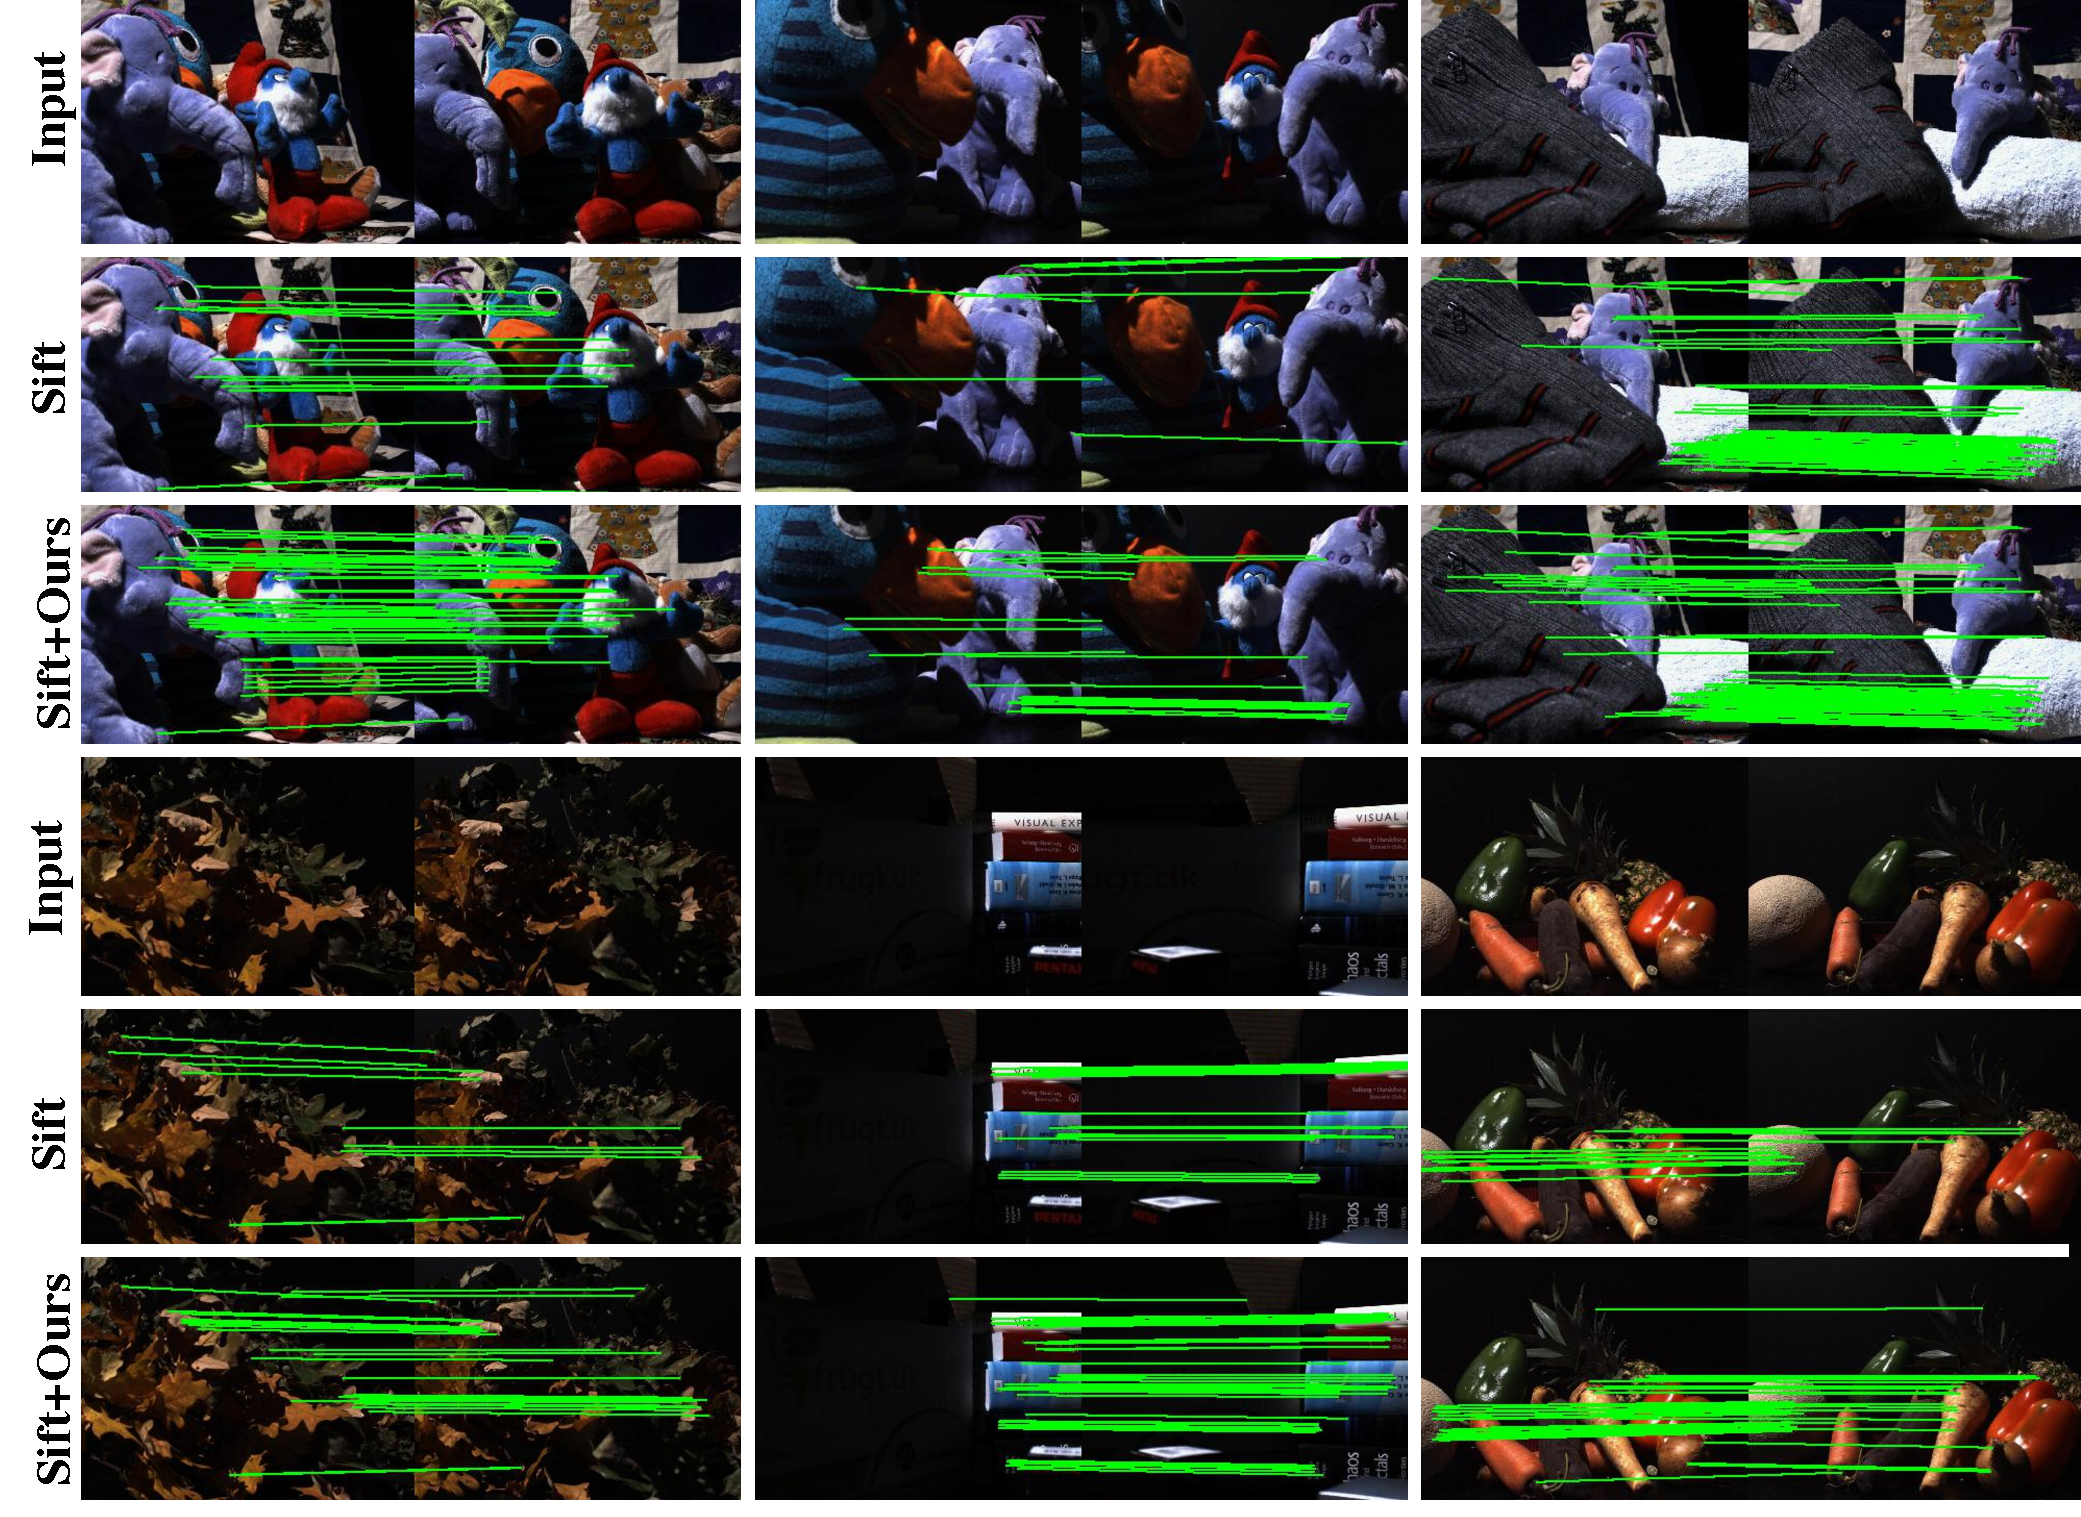
\includegraphics[width=0.8\linewidth]{FrameNet/graph/vis-sift.pdf}
    \caption{Visualize the matching between SIFT with and without our warping. With our warping, SIFT finds more correct matches.}
    \label{fig:framenet-dtu-vis}
\end{figure}
We also test the matching score as ``the ratio of ground truth correspondences that can be recovered by the whole pipeline over the number of features proposed by the pipeline in the shared viewpoint region''~\cite{yi2016lift}.

As shown in table~\ref{tab:framenet-matching}, SIFT~\cite{lowe2004distinctive} outperforms most methods. Since our method additionally reduces the perspective effects using the projected tangent principal directions, we can further improve the SIFT performance. Note that ASIFT~\cite{yu2011asift} also shares the limitation of SIFT~\cite{lowe2004distinctive} to different viewpoints, and extracts keypoints from the image with various affine transforms. Therefore, they usually provide many more correct matching but also more outliers. That is why the matching score produced by ASIFT~\cite{yu2011asift} is slightly lower than SIFT~\cite{lowe2004distinctive}. However, it sometimes shows better robustness assisted by geometric filters in certain applications.

\begin{table}
    \centering
    \tabcolsep=0.12cm
    \begin{tabular}{|c|c|c|c|}
        \hline
         SURF~\cite{bay2006surf} & ORB~\cite{rublee2011orb} & Daisy~\cite{tola2010daisy} & BRISK~\cite{leutenegger2011brisk}\\
         \hline
         .224 & .127 & .262 & .193\\
        \hline
         VGG~\cite{kahler2015very} & MatchNet~\cite{han2015matchnet} & DeepDesc~\cite{simo2015discriminative} & PN-Net~\cite{balntas2016pn}\\
         \hline
         .271 & .198 & .257 & .267\\
        \hline
         SIFT~\cite{lowe2004distinctive} & ASIFT~\cite{yu2011asift} & LIFT~\cite{yi2016lift} & SIFT+Ours\\
         \hline
         .272 & .265 & .317 & .335\\
        \hline
    \end{tabular}
    \caption{Matching score of descriptors on the DTU dataset.}
    \label{tab:framenet-matching}
\vspace{-0.2in}
\end{table}
\subsubsection{Augmented Reality}
A particularly compelling application of predicting 3D surface frames is augmented reality -- i.e., it enables adding new elements to a scene with appropriate 3D orientations.

\vspace{-0.1in}
\paragraph{Decal Attachment}  As a simple example, we investigate warping virtual decals added to RGB images based on the estimated 3D frame (first two rows of figure~\ref{fig:framenet-attach}). In our experiment, we ask the user to select one pixel in an RGB image to indicate the center point for the decal on a surface.  If we assume the surface is planar, we can compute the homography transformation required to align the decal with the scene geometry. Suppose the selected pixel is $\mb{p}$ with two estimated principal directions $\mb{i}$ and $\mb{j}$ and depth $d$. Then, the center of the pattern $(x_c,y_c)$ is located at $K^{-1}\mb{p}\cdot d$ where $K$ is the camera intrinsics. We additionally suppose that the target distance of neighboring pixels of the pattern attached to the scene is $\delta\cdot d$. Then, for pixel $(x,y)$ in the pattern, the homogeneous coordinate in the scene is
\begin{equation}
\textbf{P}(x,y) = K\cdot(K^{-1}\mb{p}\cdot d + \textbf{i}\cdot (x-x_c)\delta d + \textbf{j}\cdot (y-y_c)\delta d)\,.
\end{equation}
Therefore, the homography transform can be inferred as
\begin{equation}
    H=K[\delta \mb{i}, \delta \mb{j}, K^{-1}\mb{p} - \delta(x_c\mb{i}+y_c\mb{j})]\,.
\end{equation}
Here, $\delta$ represents the relative scale of the pattern to the depth of the pixel, which can be controlled by the user.
\begin{figure}
    \centering
    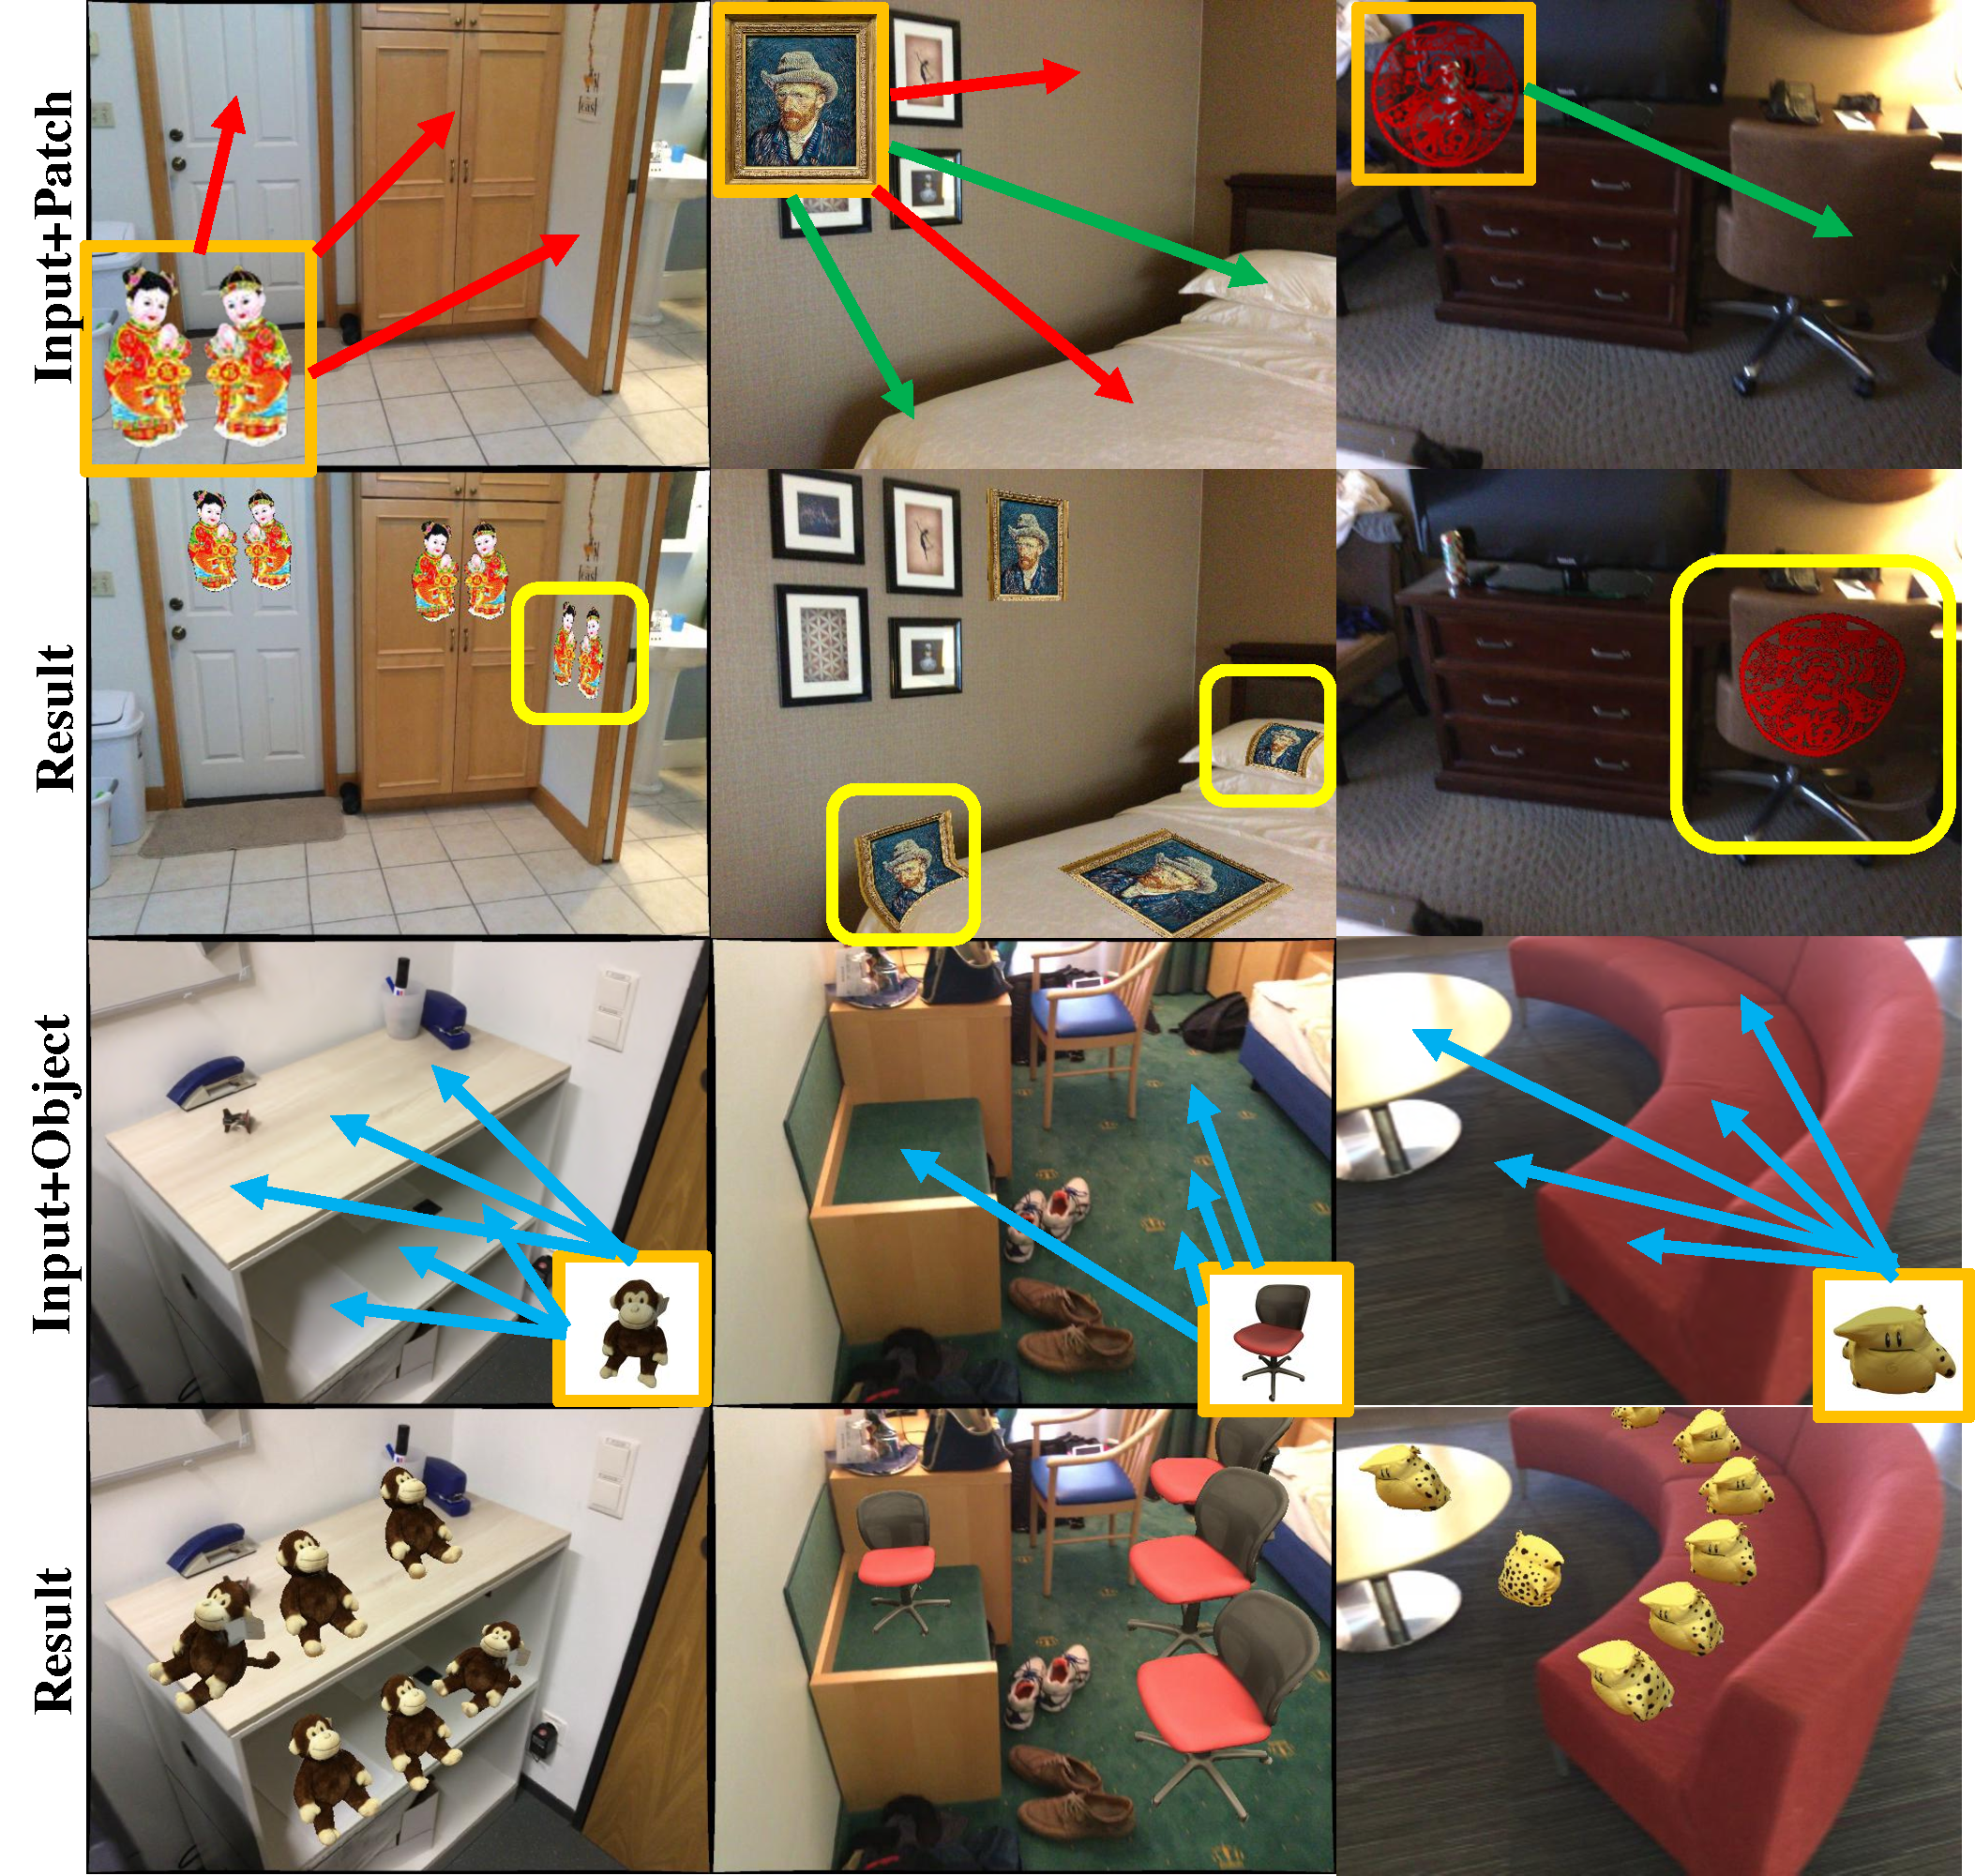
\includegraphics[width=\linewidth]{FrameNet/graph/attach.pdf}
    \caption{Adding new elements in the scene. We  use red arrows to represent rigid attachment, green to represent deformable attachment, and blue to represent object placement.}
    \label{fig:framenet-attach}
    \vspace{-0.15in}
\end{figure}
Beyond this point, our local frame even enables deformable pattern attachment on curved surfaces. Similarly, the homogeneous coordinate of any pixel $\mb{x}_t$ can be computed as
\begin{equation}
    \mb{P}(\mb{x}_t)=\mb{p} + \delta K \cdot\int_{\mb{x}_c}^{\mb{x}_t} [\textbf{i}(\mb{P}(\mb{x})),\textbf{j}(\mb{P}(\mb{x}))] d\mb{x}\,.
\end{equation}
We use the simple explicit Euler method to evolve $\mb{P}(\mb{x})$, where the path of the integration starts from the center, and follows the order guided by the breadth first search, where the expansion is from one pixel to those among its four neighbors which are not yet visited. Several examples of deformable attachment is shown in figure~\ref{fig:framenet-attach}. The user can control $\delta$ to specify the size of the attached patterns.

\vspace{-0.1in}
\paragraph{Object Placement} We can also use the local 3D frame defined by predicted principal axes to render 3D objects into RGB images, as shown in the last two rows of figure~\ref{fig:framenet-attach}.  For this application, predicting the full 3D orientation of the scene geometry is critical, so that objects can be planes not only in accordance with the surface normal, but also in the appropriate rotation around the normal (e.g., so that the front is facing the right way).   For example, the stuffed animals in the bottom left of figure~\ref{fig:framenet-attach} would appear unnatural if they were facing the wall. This could also eases mixed reality data augmentation for vision tasks, where existing methods require the depth image for plane detection~\cite{wang2019normalized}.

